 
\documentclass[a4paper,12pt]{article} % This defines  
\usepackage[top = 2.5cm, bottom = 2.5cm, left = 2.5cm, right = 2.5cm]{geometry} 

 
\usepackage[T1]{fontenc}
\usepackage[utf8]{inputenc}

\usepackage{graphicx} 
\usepackage[backend=biber,sorting=none, style=ieee]{biblatex}
\addbibresource{refe/referencias.bib}
\usepackage{setspace}
\setlength{\parindent}{0in}
\usepackage{wrapfig}

\usepackage{float}

\usepackage{xcolor}
\usepackage{colortbl}
\definecolor{udcpink}{RGB}{177,0,114}
\definecolor{udcgray}{RGB}{100,100,100}
 
\usepackage{fancyhdr}
\usepackage[breaklinks=true]{hyperref}

 \pagestyle{fancy}  

\fancyhf{} 

\lhead{\footnotesize} 

%\rhead works just like \lhead (you can also use \chead)
\rhead{\footnotesize Nuria Codesido Iglesias } %<---- Rellenar
 
\cfoot{\footnotesize \thepage} 

 \begin{document}

 \thispagestyle{empty}  

\begin{tabular}{p{15.5cm}}  
{\large \bf Hacking ético e Test de intrusión} \\ Máster Inter-Universitario en Ciberseguridad (MUNICS)  
 \\  Universidade da Coruña (UDC) y Universidade de Vigo (UVigo)\\ Curso 2024-2025  \\
\hline    
\\
\end{tabular}  
\vspace*{0.1cm}  

\begin{center}  
	{\Large \bf Práctica 2 - Identificación de vulnerabilidades
} % <---- Don't forget to put in the right number
	\vspace{1mm}
	
        % YOUR NAMES GO HERE
	{\bf Nuria Codesido Iglesias} % 
		
\end{center}  

\vspace{0.4cm}


%%%%%%%%%%%%%%%%%%%%%%%%%%%%%%%%%%%%%%%%%%%%%%%%

\renewcommand{\contentsname}{Índice} % Cambia "Contents" por "Índice"
\tableofcontents  % Genera el índice automáticamente

\newpage
\section{Identificación de CVE}
En este apartado, se realizará un análisis exhaustivo de las vulnerabilidades encontradas en las máquinas Windows y Linux, utilizando herramientas especializadas para el escaneo de vulnerabilidades como \texttt{NESSUS} y \texttt{NMAP/NSE}. Para la máquina Linux, además, se empleará \texttt{NIKTO}.

Para cada vulnerabilidad identificada, se presentará una descripción detallada, el nivel de riesgo asociado, las soluciones recomendadas y los posibles exploits que podrían ser utilizados, tanto de forma manual como automática. Si se encuentra un exploit, se proporcionará una breve descripción (en color azul). En caso de que el exploit pertenezca a una categoría de alto riesgo, como aquellos que pueden causar daños graves al sistema, se destacará en color rojo. Cabe destacar que cada exploit se buscó con la herramienta \texttt{SearchSploit} y cada búsqueda está debidamente referenciada con una imagen en el apartado \ref{Apartado2}.

 \subsection{Análisis CVE - Máquina Windows(192.168.56.6)}

\begin{table}[hp!]
  \centering
  \rowcolors{2}{white}{udcgray!25}
  \scriptsize
  \resizebox{\textwidth}{!}{
  \begin{tabular}{m{2.1cm}|m{2.6cm}|m{2cm}|m{4cm}|m{1cm}|m{3cm}|m{5cm}|m{5cm}}
  \rowcolor{udcpink!25}
 \textbf{CVE} & \textbf{Vulnerabilidad} & \textbf{Herramienta} & \textbf{Descripción} & \textbf{Riesgo} & \textbf{Solución} & \multicolumn{2}{c}{\textbf{Exploit}}  \\\hline
               &                         &                       &                       &                 &                   & \textbf{Manual} & \textbf{Automático} \\\hline

  {CVE-2017-0143} & {ETERNALBLUE (MS17-010)} & {NESSUS/ NMAP/NSE} & {Vulnerabilidad en SMBv1 que permite a un atacante remoto no autenticado ejecutar código malicioso al enviar un paquete especialmente diseñado.} & {High} & {Instalar parches específicos y deshabilitar el servicio SMBv1.} & { Microsoft Windows Server 2008 R2 (x64) - 'SrvOs2FeaToNt' SMB Remote Code Execution (MS17-010)  \ref{fig:43} \vspace{2mm} \hline \vspace{2mm} {\color{blue} \textbf{Consiste:} en aprovechar una vulnerabilidad en SMB para ejecutar código remoto en Windows Server 2008 R2. } \vspace{2mm} \hline \vspace{2mm} {\color{red} Sí, supone un peligro grave. Si el exploit se usa incorrectamente o en un sistema sin parchear, puede causar un BSOD debido a la ejecución de código en el kernel, ya que la vulnerabilidad afecta cómo SMB maneja las solicitudes de red. }} & {DOUBLEPULSAR - Payload Execution and Neutralization (Metasploit) \ref{fig:43}  \vspace{2mm} \hline \vspace{2mm} {\color{blue} \textbf{Consiste:} en permitir a un atacante ejecutar código de forma remota en sistemas Windows a través de vulnerabilidades en SMBv1.} \vspace{2mm} \hline \vspace{2mm} {\color{red} Sí, es grave. No causa BSOD, pero tiene mayor impacto por control y propagación.}}\\
  {CVE-2017-0144} & {ETERNALBLUE (MS17-010)} & {NESSUS} & {Vulnerabilidad en SMBv1 que permite a un atacante remoto no autenticado ejecutar código malicioso al enviar un paquete especialmente diseñado.} & {High} & {Instalar parches específicos y deshabilitar el servicio SMBv1.} & { Microsoft Windows Server 2008 R2 (x64) - 'SrvOs2FeaToNt' SMB Remote Code Execution (MS17-010) \ref{fig:44} \vspace{2mm} \hline \vspace{2mm} {\color{blue} \textbf{Consiste:} en aprovechar una vulnerabilidad en SMB para ejecutar código remoto en Windows Server 2008 R2.} \vspace{2mm} \hline \vspace{2mm} {\color{red} Sí, supone un peligro grave. Si el exploit se usa incorrectamente o en un sistema sin parchear, puede causar un BSOD debido a la ejecución de código en el kernel, ya que la vulnerabilidad afecta cómo SMB maneja las solicitudes de red.}} & {DOUBLEPULSAR - Payload Execution and Neutralization (Metasploit) \ref{fig:44}   \vspace{2mm} \hline \vspace{2mm} {\color{blue} \textbf{Consiste:} en permitir a un atacante ejecutar código de forma remota en sistemas Windows a través de vulnerabilidades en SMBv1.}  \vspace{2mm} \hline \vspace{2mm} {\color{red} Sí, es grave. No causa BSOD, pero tiene mayor impacto por control y propagación.}}\\
  {CVE-2017-0145} & {ETERNALBLUE (MS17-010)} & {NESSUS} & {Vulnerabilidad en SMBv1 que permite a un atacante remoto no autenticado ejecutar código malicioso al enviar un paquete especialmente diseñado.} & {High} & {Instalar parches específicos y deshabilitar el servicio SMBv1.} & {Microsoft Windows Server 2008 R2 (x64) - 'SrvOs2FeaToNt' SMB Remote Code Execution (MS17-010) \ref{fig:45} \vspace{2mm} \hline \vspace{2mm} {\color{blue} \textbf{Consiste:} en aprovechar una vulnerabilidad en SMB para ejecutar código remoto en Windows Server 2008 R2.} \vspace{2mm} \hline \vspace{2mm} {\color{red} Sí, supone un peligro grave. Si el exploit se usa incorrectamente o en un sistema sin parchear, puede causar un BSOD debido a la ejecución de código en el kernel, ya que la vulnerabilidad afecta cómo SMB maneja las solicitudes de red. }} & {DOUBLEPULSAR - Payload Execution and Neutralization (Metasploit) \ref{fig:45}   \vspace{2mm} \hline \vspace{2mm} {\color{blue} \textbf{Consiste:} en permitir a un atacante ejecutar código de forma remota en sistemas Windows a través de vulnerabilidades en SMBv1.} \vspace{2mm} \hline \vspace{2mm} {\color{red} Sí, es grave. No causa BSOD, pero tiene mayor impacto por control y propagación.}}\\
  {CVE-2017-0146} & {ETERNALBLUE (MS17-010)} & {NESSUS} & {Vulnerabilidad en SMBv1 que permite a un atacante remoto no autenticado ejecutar código malicioso al enviar un paquete especialmente diseñado.} & {High} & {Instalar parches específicos y deshabilitar el servicio SMBv1.} & { Microsoft Windows Server 2008 R2 (x64) - 'SrvOs2FeaToNt' SMB Remote Code Execution (MS17-010) \ref{fig:46} \vspace{2mm} \hline \vspace{2mm} {\color{blue} \textbf{Consiste:} en aprovechar una vulnerabilidad en SMB para ejecutar código remoto en Windows Server 2008 R2.} \vspace{2mm} \hline \vspace{2mm} {\color{red} Sí, supone un peligro grave. Si el exploit se usa incorrectamente o en un sistema sin parchear, puede causar un BSOD debido a la ejecución de código en el kernel, ya que la vulnerabilidad afecta cómo SMB maneja las solicitudes de red.}} & {DOUBLEPULSAR - Payload Execution and Neutralization (Metasploit) \ref{fig:46}  \vspace{2mm} \hline \vspace{2mm} {\color{blue} \textbf{Consiste:} en permitir a un atacante ejecutar código de forma remota en sistemas Windows a través de vulnerabilidades en SMBv1.} \vspace{2mm} \hline \vspace{2mm} {\color{red} Sí, es grave. No causa BSOD, pero tiene mayor impacto por control y propagación.}}\\
  {CVE-2017-0147} & {ETERNALBLUE (MS17-010)} & {NESSUS} & {Vulnerabilidad en SMBv1 que permite a un atacante remoto no autenticado revelar información sensible mediante un paquete especialmente diseñado.} & {High} & {Instalar parches específicos y deshabilitar el servicio SMBv1.} & { Microsoft Windows Server 2008 R2 (x64) - 'SrvOs2FeaToNt' SMB Remote Code Execution (MS17-010) \ref{fig:47} \vspace{2mm} \hline \vspace{2mm} {\color{blue} \textbf{Consiste:} en aprovechar una vulnerabilidad en SMB para ejecutar código remoto en Windows Server 2008 R2.} \vspace{2mm} \hline \vspace{2mm} {\color{red} Sí, supone un peligro grave. Si el exploit se usa incorrectamente o en un sistema sin parchear, puede causar un BSOD debido a la ejecución de código en el kernel, ya que la vulnerabilidad afecta cómo SMB maneja las solicitudes de red.}} & {DOUBLEPULSAR - Payload Execution and Neutralization (Metasploit) \ref{fig:47}  \vspace{2mm} \hline \vspace{2mm} {\color{blue} \textbf{Consiste:} en permitir a un atacante ejecutar código de forma remota en sistemas Windows a través de vulnerabilidades en SMBv1.} \vspace{2mm} \hline \vspace{2mm} {\color{red} Sí, es grave. No causa BSOD, pero tiene mayor impacto por control y propagación.}}\\

  
  \end{tabular}}
  \caption{Identificación de CVE - Windows(192.168.56.6)}
  \label{tab:windows1}
\end{table}

\newpage

\begin{table}[hp!]
  \centering
  \rowcolors{2}{white}{udcgray!25}
  \scriptsize
  \resizebox{\textwidth}{!}{
  \begin{tabular}{m{2.1cm}|m{2.6cm}|m{2cm}|m{4cm}|m{1cm}|m{3cm}|m{5cm}|m{5cm}}
  \rowcolor{udcpink!25}
 \textbf{CVE} & \textbf{Vulnerabilidad} & \textbf{Herramienta} & \textbf{Descripción} & \textbf{Riesgo} & \textbf{Solución} & \multicolumn{2}{c}{\textbf{Exploit}}  \\\hline
               &                         &                       &                       &                 &                   & \textbf{Manual} & \textbf{Automático} \\\hline

      {CVE-2017-0148} & {ETERNALBLUE (MS17-010)} & {NESSUS} & {Vulnerabilidad en SMBv1 que permite a un atacante remoto no autenticado ejecutar código malicioso al enviar un paquete especialmente diseñado.} & {High} & {Instalar parches específicos y deshabilitar el servicio SMBv1.} & { Microsoft Windows Server 2008 R2 (x64) - 'SrvOs2FeaToNt' SMB Remote Code Execution (MS17-010) \ref{fig:48}  \vspace{2mm} \hline \vspace{2mm} {\color{blue} \textbf{Consiste:} en aprovechar una vulnerabilidad en SMB para ejecutar código remoto en Windows Server 2008 R2. Aunque no causa un BSOD, permite tomar control del sistema y puede ser utilizado para propagar malware } \vspace{2mm} \hline \vspace{2mm} {\color{red} Sí, supone un peligro grave. Si el exploit se usa incorrectamente o en un sistema sin parchear, puede causar un BSOD debido a la ejecución de código en el kernel, ya que la vulnerabilidad afecta cómo SMB maneja las solicitudes de red.}} & {DOUBLEPULSAR - Payload Execution and Neutralization (Metasploit) \ref{fig:48} \vspace{2mm} \hline \vspace{2mm} {\color{blue} \textbf{Consiste:} en permitir a un atacante ejecutar código de forma remota en sistemas Windows a través de vulnerabilidades en SMBv1.} \vspace{2mm} \hline \vspace{2mm} {\color{red} Sí, es grave. No causa BSOD, pero tiene mayor impacto por control y propagación.}}\\

      {CVE-2016-0128} & {Elevación de privilegios en SAM y LSAD (MS16-047)} & {NESSUS} & {Vulnerabilidad en los protocolos SAM y LSAD que permite la elevación de privilegios mediante la manipulación de la autenticación sobre RPC, permitiendo el acceso al SAM.} & {Medium} & {Aplicar los parches de seguridad de Microsoft para las versiones afectadas de Windows.} & {No Results \ref{fig:16No}} & {No Results \ref{fig:16No}}\\

%hacen falta?
  {CVE-2010-2730} & {Desbordamiento de búfer} & {NMAP} & {Vulnerabilidad en Outlook que permite ejecución remota de código} & {High} & {Aplicar parche de seguridad de Microsoft} & {No Results \ref{fig:16No}} & {No Results \ref{fig:16No}} \\
  {CVE-2010-3972} & {Ejecución remota de código} & {NMAP} & {Fallo en el motor de script de IE que permite ejecución arbitraria de código} & {High} & {Actualizar Internet Explorer} & {Microsoft IIS 7.5 (Windows 7) - FTPSVC Unauthorized Remote Denial of Service (PoC) \ref{fig:1072} \vspace{2mm} \hline \vspace{2mm} {\color{blue} \textbf{Consiste} en aprovechar un desbordamiento de búfer en el servicio FTP al procesar ciertos comandos FTP, lo que puede hacer que el servicio deje de responder }} & {No Results \ref{fig:1072}} \\
  {CVE-2010-1899} & {Corrupción de memoria} & {NMAP} & {Fallo en OpenType Font Driver que permite ejecución de código} & {Medium} & {Aplicar actualizaciones de seguridad} & { Microsoft IIS 6.0 - ASP Stack Overflow Stack Exhaustion (Denial of Service) (MS10-065) \ref{fig:1089} \vspace{2mm} \hline \vspace{2mm} {\color{blue} \textbf{Consiste} en aprovechar un desbordamiento de pila al procesar solicitudes POST con muchos parámetros, lo que hace que el servidor se vuelva no responsivo hasta que se reinicie manualmente}} & {No Results \ref{fig:1089}}\\
  {CVE-2020-1113} & {Elevación de privilegios	} & {NMAP} & {Fallo en el servicio de actualización que permite escalación de privilegios} & {High} & {Instalar parches de seguridad de Microsoft}  & {No Results \ref{fig:20No}} & {No Results \ref{fig:20No}}\\
  {CVE-2018-7445} & {Desbordamiento de memoria} & {NMAP} & {Vulnerabilidad en VLC que puede provocar ejecución de código malicioso} & {Critical} & {Actualizar VLC a la última versión}  & {MikroTik RouterOS < 6.41.3/6.42rc27 - SMB Buffer Overflow  \ref{fig:1845} \vspace{2mm} \hline \vspace{2mm} {\color{blue} \textbf{Consiste} en aprovechar un desbordamiento de búfer al procesar mensajes de solicitud de sesión NetBIOS, permitiendo la ejecución de código sin autenticación } \vspace{2mm} \hline \vspace{2mm} {\color{red} Sí, es un peligro grave, ya que permite ejecución remota de código. No provoca un BSOD, pero puede tomar control del enrutador, afectando la red.}} & {No Results \ref{fig:1845}} \\
               
  \end{tabular}}
  \caption{Identificación de CVE 2 - Windows(192.168.56.6)}
  \label{tab:windows2}
\end{table}

 \newpage
 \subsection{Análisis CVE - Máquina Linux (192.168.56.9)}

\begin{table}[hp!]
  \centering
  \rowcolors{2}{white}{udcgray!25}
  \scriptsize
  \resizebox{\textwidth}{!}{
  \begin{tabular}{m{2.1cm}|m{2.6cm}|m{2cm}|m{4cm}|m{1cm}|m{3cm}|m{5cm}|m{5cm}}
  \rowcolor{udcpink!25}
 \textbf{CVE} & \textbf{Vulnerabilidad} & \textbf{Herramienta} & \textbf{Descripción} & \textbf{Riesgo} & \textbf{Solución} & \multicolumn{2}{c}{\textbf{Exploit}}  \\\hline
               &                         &                       &                       &                 &                   & \textbf{Manual} & \textbf{Automático} \\\hline

  {CVE-2008-0166} & {Debian OpenSSH/OpenSSL Package Random Number Generator Weakness (SSL check)} & {NESSUS} & {El generador de números aleatorios de OpenSSL en Debian/Ubuntu es débil, permitiendo la predicción de claves privadas y ataques MITM.} & {Critical} & {Regenerar todas las claves criptográficas SSH, SSL y OpenVPN.} & {OpenSSL 0.9.8c-1 < 0.9.8g-9 (Debian and Derivatives) - Predictable PRNG Brute Force SSH (Ruby) \ref{fig:linux1} \vspace{2mm} \hline \vspace{2mm} {\color{blue} \textbf{Consiste}  en permitir a un atacante predecir números aleatorios generados por OpenSSL, facilitando un ataque de fuerza bruta contra claves SSH en servidores vulnerables}} & {No results \ref{fig:linux1}}\\
  {CVE-2008-0166} & {Debian OpenSSH/OpenSSL Package Random Number Generator Weakness} & {NESSUS} & {Claves SSH generadas en Debian/Ubuntu pueden ser fácilmente descubiertas y usadas para ataques.} & {Critical} & {Regenerar todas las claves SSH en el host afectado.} & {OpenSSL 0.9.8c-1 < 0.9.8g-9 (Debian and Derivatives) - Predictable PRNG Brute Force SSH (Ruby) \ref{fig:linux1} \vspace{2mm} \hline \vspace{2mm} {\color{blue} \textbf{Consiste}  en permitir a un atacante predecir números aleatorios generados por OpenSSL, facilitando un ataque de fuerza bruta contra claves SSH en servidores vulnerables}} & {No results \ref{fig:linux1}}\\
  {CVE-2020-1745} & {Apache Tomcat AJP Connector Request Injection (Ghostcat)} & {NESSUS} & {Un atacante remoto puede leer archivos de aplicaciones web y ejecutar código si el servidor permite la carga de archivos.} & {High} & {Configurar autorización en el conector AJP y actualizar Tomcat a 7.0.100, 8.5.51 o 9.0.31 o posterior.} & {Seowon SLR-120 Router - Remote Code Execution (Unauthenticated) \ref{fig:linux2} \vspace{2mm} \hline \vspace{2mm} {\color{blue} \textbf{Consiste} en afectar a los enrutadores Seowon SLR-120 y permite ejecución remota de código sin autenticación }} & {No Results \ref{fig:linux2}}\\
  {CVE-2020-1938} & {Apache Tomcat AJP Connector Request Injection (Ghostcat)} & {NESSUS/NMAP} & {Similar a CVE-2020-1745, permite la lectura de archivos y ejecución de código en servidores vulnerables.} & {High} & {Configurar autorización en el conector AJP y actualizar Tomcat.} & { No Results \ref{fig:linux3}} & { Apache Tomcat - AJP 'Ghostcat' File Read/Inclusion (Metasploit)  \ref{fig:linux3} \vspace{2mm} \hline \vspace{2mm} {\color{blue} \textbf{Consiste} en permitir a un atacante remoto y no autenticado leer archivos de aplicaciones web o incluir archivos maliciosos para ejecutar código en el servido.}}\\
  {CVE-2016-2183} & {SSL Medium Strength Cipher Suites Supported (SWEET32)} & {NESSUS} & {El servicio remoto permite el uso de cifrados SSL de fortaleza media (3DES), lo que facilita ataques criptográficos.} & {Medium} & {Reconfigurar la aplicación para evitar el uso de estos cifrados.} & {No Results \ref{fig:linux4}}  & {No Results \ref{fig:linux4}}\\
  {CVE-2013-2566} & {SSL RC4 Cipher Suites Supported (Bar Mitzvah)} & {NESSUS} & {Uso del cifrado RC4, que tiene sesgos predecibles y puede ser descifrado si se capturan suficientes datos.} & {Medium} & {Deshabilitar el uso de RC4 y configurar TLS 1.2 con AES-GCM.} & {No Results \ref{fig:linux5}}  & {No Results \ref{fig:linux5}}\\
  {CVE-2015-2808} & {SSL RC4 Cipher Suites Supported (Bar Mitzvah)} & {NESSUS} & {Similar a CVE-2013-2566, afecta la seguridad de los datos transmitidos.} & {Medium} & {Reconfigurar la aplicación para evitar el uso de RC4.}  & {No Results \ref{fig:linux6}}  & {No Results \ref{fig:linux6}}\\
  {CVE-1999-0651} & {rlogin Service Detection} & {NESSUS/NMAP} & {El servicio rlogin está en ejecución en el host remoto, transmitiendo datos en texto plano, lo que permite ataques Man-in-the-Middle y posibles accesos no autenticados.} & {High} & {Comentar la línea 'login' en \texttt{/etc/inetd.conf} y reiniciar inetd, o deshabilitar rlogin y usar SSH.}  & {No Results \ref{fig:linux7}}  & {No Results \ref{fig:linux7}}\\
  {CVE-2016-0800} & {SSL DROWN Attack} & {NESSUS} & {El host admite SSLv2, lo que permite un ataque de oracle de relleno Bleichenbacher para descifrar tráfico TLS capturado.} & {Medium} & {Deshabilitar SSLv2 y cifrados de grado de exportación, asegurando que las claves privadas no se usen con servidores SSLv2.}  & {No Results \ref{fig:linux8}}  & {No Results \ref{fig:linux8}}\\
  {CVE-2016-2118} & {Samba Badlock Vulnerability} & {NESSUS} & {Vulnerabilidad en Samba que permite a un atacante interceptar y degradar la autenticación en el protocolo RPC, pudiendo modificar datos sensibles en Active Directory.} & {Medium} & {Actualizar Samba a la versión 4.2.11 / 4.3.8 / 4.4.2 o posterior.}  & {No Results \ref{fig:linux9}}  & {No Results \ref{fig:linux9}}\\
  {CVE-2020-8616} & {ISC BIND Service Downgrade / Reflected DoS} & {NESSUS} & {ISC BIND 9 permite realizar demasiadas búsquedas al procesar una respuesta de referencia, lo que puede ser explotado para degradar el rendimiento del servidor o para ataques de reflexión.} & {Medium} & {Actualizar ISC BIND a la versión recomendada por el proveedor.}  & {No Results \ref{fig:linux10}}  & {No Results \ref{fig:linux10}}\\
  {CVE-2003-1567} & {HTTP TRACE / TRACK Methods Allowed} & {NESSUS} & {El servidor web remoto permite los métodos TRACE y TRACK, lo que puede ser utilizado para ataques de cross-site tracing (XST).} & {Medium} & {Deshabilitar los métodos TRACE y TRACK en la configuración del servidor web.}  & {No Results \ref{fig:linux11}}  & {No Results \ref{fig:linux11}}\\
  {CVE-2004-2320} & {HTTP TRACE / TRACK Methods Allowed} & {NESSUS} & {El servidor web remoto permite los métodos TRACE y TRACK, lo que puede ser utilizado para ataques de cross-site tracing (XST).} & {Medium} & {Deshabilitar los métodos TRACE y TRACK en la configuración del servidor web.}  & {No Results \ref{fig:linux12}}  & {No Results \ref{fig:linux12}}\\
  {CVE-2010-0386} & {HTTP TRACE / TRACK Methods Allowed} & {NESSUS} & {El servidor web remoto permite los métodos TRACE y TRACK, lo que puede ser utilizado para ataques de cross-site tracing (XST).} & {Medium} & {Deshabilitar los métodos TRACE y TRACK en la configuración del servidor web.}  & {No Results \ref{fig:linux13}}  & {No Results \ref{fig:linux13}}\\
  
  \end{tabular}}
  \caption{Identificación de CVE - Linux(192.168.56.9)}
  \label{tab:linux1}
\end{table}

\newpage

\begin{table}[hp!]
  \centering
  \rowcolors{2}{white}{udcgray!25}
  \scriptsize
  \resizebox{\textwidth}{!}{
  \begin{tabular}{m{2.1cm}|m{2.6cm}|m{2cm}|m{4cm}|m{1cm}|m{3cm}|m{5cm}|m{5cm}}
  \rowcolor{udcpink!25}
 \textbf{CVE} & \textbf{Vulnerabilidad} & \textbf{Herramienta} & \textbf{Descripción} & \textbf{Riesgo} & \textbf{Solución} & \multicolumn{2}{c}{\textbf{Exploit}}  \\\hline
               &                         &                       &                       &                 &                   & \textbf{Manual} & \textbf{Automático} \\\hline
  
  {CVE-2007-1858} & {SSL Anonymous Cipher Suites Supported} & {NESSUS} & {El servicio remoto admite cifrados SSL anónimos, lo que permite ataques de Man-in-the-Middle debido a la falta de autenticación.} & {Low} & {Reconfigurar la aplicación para evitar el uso de cifrados débiles.} & {No Results \ref{fig:linux14}}  & {No Results \ref{fig:linux14}}\\
  {CVE-2011-0411} & {SMTP Service STARTTLS Plaintext Command Injection} & {NESSUS} & {Implementación defectuosa de STARTTLS en el servicio SMTP permite a un atacante inyectar comandos en la fase de texto plano y ejecutarlos en la fase cifrada, lo que puede llevar al robo de correos electrónicos o credenciales SASL.} & {Medium} & {Contactar al proveedor para obtener una actualización.} & {No Results \ref{fig:linux14}}  & {No Results \ref{fig:linux14}}\\
  {CVE-2011-1430} & {SMTP Service STARTTLS Plaintext Command Injection} & {NESSUS} & {Implementación defectuosa de STARTTLS en el servicio SMTP permite a un atacante inyectar comandos en la fase de texto plano y ejecutarlos en la fase cifrada, lo que puede llevar al robo de correos electrónicos o credenciales SASL.} & {Medium} & {Contactar al proveedor para obtener una actualización.} & {No Results \ref{fig:linux14}}  & {No Results \ref{fig:linux14}}\\
  {CVE-2011-1431} & {SMTP Service STARTTLS Plaintext Command Injection} & {NESSUS} & {Implementación defectuosa de STARTTLS en el servicio SMTP permite a un atacante inyectar comandos en la fase de texto plano y ejecutarlos en la fase cifrada, lo que puede llevar al robo de correos electrónicos o credenciales SASL.} & {Medium} & {Contactar al proveedor para obtener una actualización.} & {No Results \ref{fig:linux14}}  & {No Results \ref{fig:linux14}}\\
  {CVE-2011-1432} & {SMTP Service STARTTLS Plaintext Command Injection} & {NESSUS} & {Implementación defectuosa de STARTTLS en el servicio SMTP permite a un atacante inyectar comandos en la fase de texto plano y ejecutarlos en la fase cifrada, lo que puede llevar al robo de correos electrónicos o credenciales SASL.} & {Medium} & {Contactar al proveedor para obtener una actualización.} & {No Results \ref{fig:linux14}}  & {No Results \ref{fig:linux14}}\\
  {CVE-2011-1506} & {SMTP Service STARTTLS Plaintext Command Injection} & {NESSUS} & {Implementación defectuosa de STARTTLS en el servicio SMTP permite a un atacante inyectar comandos en la fase de texto plano y ejecutarlos en la fase cifrada, lo que puede llevar al robo de correos electrónicos o credenciales SASL.} & {Medium} & {Contactar al proveedor para obtener una actualización.} & {No Results \ref{fig:linux14}}  & {No Results \ref{fig:linux14}}\\
  {CVE-2011-2165} & {SMTP Service STARTTLS Plaintext Command Injection} & {NESSUS} & {Implementación defectuosa de STARTTLS en el servicio SMTP permite a un atacante inyectar comandos en la fase de texto plano y ejecutarlos en la fase cifrada, lo que puede llevar al robo de correos electrónicos o credenciales SASL.} & {Medium} & {Contactar al proveedor para obtener una actualización.} & {Watchguard XCS 10.0 - Multiple Vulnerabilities \ref{fig:linux15} \vspace{2mm} \hline \vspace{2mm} {\color{blue} \textbf{Consiste} en permitir inyección de SQL, ejecución de comandos y escalada de privilegios.}}  & {No Results \ref{fig:linux15}}\\
  {CVE-2015-0204} & {SSL/TLS EXPORT\_RSA <= 512-bit Cipher Suites Supported (FREAK)} & {NESSUS} & {El host admite cifrados EXPORT\_RSA con claves de 512 bits o menos, lo que permite a un atacante factorizar la clave y descifrar el tráfico SSL/TLS.} & {High} & {Deshabilitar los cifrados EXPORT\_RSA y actualizar la configuración de TLS} & {No Results \ref{fig:linux16}}  & {No Results \ref{fig:linux16}}\\
  {CVE-2020-8617} & {ISC BIND Denial of Service} & {NESSUS} & {Vulnerabilidad en ISC BIND que permite un ataque DoS mediante un mensaje especialmente diseñado.} & {Medium} & {Actualizar a la versión corregida más cercana a la versión actual de BIND.} & {BIND - 'TSIG' Denial of Service \ref{fig:linux17}  \vspace{2mm} \hline \vspace{2mm} {\color{blue} \textbf{Consiste} en provocar un Denial of Service (DoS) en servidores BIND al enviar consultas DNS manipuladas con TSIG  malformadas. }}  & {No Results \ref{fig:linux17}} \\
  {CVE-2020-8622} & {ISC BIND DoS (TSIG-signed request)} & {NESSUS} & {DoS en ISC BIND al verificar una respuesta truncada a una solicitud TSIG, permitiendo el cierre del servidor.} & {Medium} & {Actualizar a BIND 9.11.22, 9.16.6, 9.17.4 o posterior.} & {No Results \ref{fig:linux18}}  & {No Results \ref{fig:linux18}}\\
  {CVE-2014-3566} & {SSLv3 POODLE Vulnerability} & {NESSUS/ NMAP/NSE} & {Vulnerabilidad en SSLv3 que permite ataques MitM para descifrar información confidencial.} & {Medium} & {Deshabilitar SSLv3 y habilitar el mecanismo TLS Fallback SCSV.} & {No Results \ref{fig:linux18}}  & {No Results \ref{fig:linux18}}\\

  \end{tabular}}
  \caption{Identificación de CVE 2 - Linux(192.168.56.9)}
  \label{tab:linux2}
\end{table}


\begin{table}[hp!]
  \centering
  \rowcolors{2}{white}{udcgray!25}
  \scriptsize
  \resizebox{\textwidth}{!}{
  \begin{tabular}{m{2.1cm}|m{2.6cm}|m{2cm}|m{4cm}|m{1cm}|m{3cm}|m{5cm}|m{5cm}}
  \rowcolor{udcpink!25}
 \textbf{CVE} & \textbf{Vulnerabilidad} & \textbf{Herramienta} & \textbf{Descripción} & \textbf{Riesgo} & \textbf{Solución} & \multicolumn{2}{c}{\textbf{Exploit}}  \\\hline
               &                         &                       &                       &                 &                   & \textbf{Manual} & \textbf{Automático} \\\hline

  {CVE-1999-0524} & {ICMP Timestamp Request Remote Date Disclosure} & {NESSUS} & {Permite a un atacante conocer la fecha y hora del sistema, útil para evadir autenticación basada en tiempo.} & {Low} & {Filtrar solicitudes ICMP timestamp (13) y respuestas (14).} & {No Results \ref{fig:linux18}}  & {No Results \ref{fig:linux18}}\\
  {CVE-2008-5161} & {SSH Server CBC Mode Ciphers Enabled} & {NESSUS/NMAP} & {Uso de cifrados CBC en SSH, lo que puede permitir la recuperación de texto en claro.} & {Low} & {Deshabilitar CBC y habilitar modos CTR o GCM.} & {No Results \ref{fig:linux18}}  & {No Results \ref{fig:linux18}}\\
  {CVE-2015-4000} & {SSL/TLS EXPORT\_DHE <= 512-bit Export Cipher Suites (Logjam)} & {NESSUS/NMAP} & {Uso de claves Diffie-Hellman débiles en SSL/TLS, permitiendo ataque de downgrade.} & {Low} & {Eliminar soporte para EXPORT\_DHE en la configuración del servicio.} & {No Results \ref{fig:linux18}}  & {No Results \ref{fig:linux18}}\\
  {CVE-2015-4000} & {SSL/TLS Diffie-Hellman Modulus <= 1024 Bits (Logjam)} & {NESSUS/NMAP} & {Uso de claves Diffie-Hellman de ≤1024 bits, permitiendo ataque de fuerza bruta en corto tiempo.} & {Low} & {Usar módulos Diffie-Hellman de al menos 2048 bits.} & {No Results \ref{fig:linux18}}  & {No Results \ref{fig:linux18}}\\
  {CVE-1999-0678} & {Exposición de directorios sensibles} & {NIKTO} & {(puerto 80) - vulnerabilidad que permite a los atacantes exploren directorios sensibles (como /usr/doc) a través de la indexación de directorios en un servidor web.} & {Medium} & {Deshabilitar la indexación de directorios en el servidor web, asegurándose de que no haya directorios sensibles accesibles sin autenticación. También es recomendable restringir el acceso a archivos sensibles en el servidor.} & {Debian 2.1 - HTTPd \ref{fig:linux19} \vspace{2mm} \hline \vspace{2mm} {\color{blue} \textbf{Consiste} en permitir a un atacante remoto ejecutar comandos arbitrarios en el servidor debido a una incorrecta configuración del servidor web. } \vspace{2mm} \hline \vspace{2mm} {\color{red} Sí, supone un peligro grave.No provoca un BSOD, pero permite ejecución remota de comandos. }}  & {No Results \ref{fig:linux19}}\\
  {CVE-2003-1418} & {Tomcat Directory Traversal} & {NIKTO} & {(puerto 80) - vulnerabilidad de directory traversal en Apache Tomcat que permite a un atacante acceder a archivos arbitrarios fuera del directorio web.} & {Medium} & {Limitar el acceso a archivos sensibles y asegurarse de que las rutas solicitadas no sean manipulables y actualizar Apache.} & {No Results \ref{fig:linux20}}  & {No Results \ref{fig:linux20}}\\
  {CVE-2000-0672} & {Tomcat Arbitrary File Reading} & {NIKTO} & {(puerto 8180) - vulnerabilidad de Apache Tomcat que permite a un atacante acceder y leer archivos arbitrarios en el servidor.} & {Medium} & {Actualizar a versiones de Tomcat que no presenten esta vulnerabilidad y restringir el acceso a las rutas sensibles.}  & {No Results \ref{fig:linux20}}  & {No Results \ref{fig:linux20}}\\

  {CVE-2011-2523} & {Backdoor en vsftpd 2.3.4} & {NMAP/NSE} & {Shell abierto en puerto 6200/tcp.} & {Critical} & {Actualizar vsftpd a versión segura.} & {vsftpd 2.3.4 - Backdoor Command Execution \ref{fig:linux21} \vspace{2mm} \hline \vspace{2mm} {\color{blue} \textbf{Consiste} en permitir a un atacante ejecute comandos arbitrarios en el sistema mediante un backdoor presente en una versión específica de vsftpd. } \vspace{2mm} \hline \vspace{2mm} {\color{red} Sí, supone un peligro grave.No provoca un BSOD, pero permite ejecución remota de comandos. }}  & {vsftpd 2.3.4 - Backdoor Command Execution (Metasploit)  \ref{fig:linux21} \vspace{2mm} \hline \vspace{2mm} {\color{blue} \textbf{Consiste} en permitir a un atacante ejecute comandos arbitrarios en el sistema mediante un backdoor presente en una versión específica de vsftpd. } \vspace{2mm} \hline \vspace{2mm} {\color{red} Sí, supone un peligro grave.No provoca un BSOD, pero permite ejecución remota de comandos. }}\\
  
  {CVE-2007-6750} & {Denegación de servicio en Apache HTTP Server (Slowloris)} & {NMAP/NSE} & {Ataque que mantiene conexiones abiertas con solicitudes HTTP parciales, agotando recursos del servidor.} & {Medium} & {Actualizar Apache a la versión 2.2.15 o superior.} & {No Results \ref{fig:linux22}}  & {No Results \ref{fig:linux22}} \\

  %hacen falta?
  {CVE-2005-2040} & {Desbordamiento de búfer} & {NMAP} & {Vulnerabilidad en Samba que permite ejecución remota de código} & {Medium} & {Actualizar Samba} & {No Results \ref{fig:linux23}}  & {No Results \ref{fig:linux23}}\\
  {CVE-2008-0122} & {Desbordamiento de búfer} & {NMAP} & {Vulnerabilidad en Flash Player que permite ejecución de código} & {High} & {Actualizar o eliminar Flash Player}  & {No Results \ref{fig:linux23}}  & {No Results \ref{fig:linux23}} \\
  {CVE-2017-3167} & {Autenticación débil} & {NMAP} & {Fallo en la autenticación de Apache que permite ataques de fuerza bruta} & {Critical} & {Aplicar parches y reforzar autenticación}  & {No Results \ref{fig:linux23}}  & {No Results \ref{fig:linux23}} \\
  {CVE-2017-8779} & {Desbordamiento de pila} & {NMAP} & {Fallo en Putty que permite ejecución de código malicioso} & {High} & {Actualizar Putty} & {   RPCBind / libtirpc - Denial of Service \ref{fig:linux24} \vspace{2mm} \hline \vspace{2mm} {\color{blue} \textbf{Consiste} en permitir a un atacante enviar paquetes UDP al puerto 111, lo que puede causar el consumo excesivo de memoria y la interrupción de servicios.}} & { No Results \ref{fig:linux24}} \\
  {CVE-2023-42670} & {Cross-Site Scripting (XSS)} & {NMAP} & {Falta de validación en entrada permite inyección de scripts} & {Medium} & {Aplicar filtros de validación y escape de caracteres} & {No Results \ref{fig:linux25}} & { No Results \ref{fig:linux25}} \\
  {CVE-1999-0502} & {Contraseña débil} & {NMAP} & {Uso de contraseñas predeterminadas o débiles en sistemas} & {High} & {Aplicar políticas de contraseñas seguras}   & {No Results \ref{fig:linux26}} & { SSH - User Code Execution (Metasploit)  \ref{fig:linux26} \vspace{2mm} \hline \vspace{2mm} {\color{blue} \textbf{Consiste} en permitir la ejecución de código de usuario a través de SSH.} \vspace{2mm} \hline \vspace{2mm} {\color{red} Sí, supone un peligro grave, pero no causa un BSOD. En cambio, permite a un atacante obtener acceso no autorizado al sistema.}}\\
  {CVE-1999-1126} & {Inyección de comandos} & {NMAP} & {Uso de caracteres especiales en entradas no validadas} & {Low} & {Implementar validaciones de entrada} & {No Results \ref{fig:linux27}} & { No Results \ref{fig:linux27}} \\
  {CVE-2011-3556} & {Desbordamiento de memoria} & {NMAP} & {Vulnerabilidad en Java que permite ejecución remota de código} & {High} & {Actualizar Java Runtime} & {No Results \ref{fig:linux28}} & { Java RMI - Server Insecure Default Configuration Java Code Execution (Metasploit)\ref{fig:linux28} \vspace{2mm} \hline \vspace{2mm} {\color{blue} \textbf{Consiste} en permitir a un atacante ejecutar código remoto en el servidor afectado sin autenticación.} \vspace{2mm} \hline \vspace{2mm} {\color{red} Sí, supone un peligro grave, pero no causa un BSOD. En cambio, permite la ejecución remota de código.}}\\
  {CVE-2009-0543} & {Denegación de servicio (DoS)} & {NMAP} & {Falla en IIS que permite ataques de denegación de servicio} & {Medium} & {Aplicar actualizaciones de seguridad} & { ProFTPd - 'mod\_mysql' Authentication Bypass \ref{fig:linux28} \hline \vspace{2mm} {\color{blue} \textbf{Consiste} en permitir eludir la autenticación mediante una inyección SQL. }} & { No Results \ref{fig:linux29}}\\
  {CVE-2008-4097} & {Desbordamiento de pila} & {NMAP} & {Vulnerabilidad en VLC que permite ejecución de código arbitrario} & {Medium} & {Actualizar VLC a la última versión} & { No Results \ref{fig:linux30}}& { No Results \ref{fig:linux30}} \\
  {CVE-2010-1447} & {Corrupción de memoria} & {NMAP} & {Fallo en el kernel de Windows que permite escalación de privilegios} & {High} & {Aplicar parches de seguridad} & { No Results \ref{fig:linux30}}& { No Results \ref{fig:linux30}}\\
  {CVE-2002-1511} & {Inyección SQL} & {NMAP} & {Falta de validación en entradas permite inyección SQL} & {Medium} & {Aplicar validaciones en consultas SQL} & { No Results \ref{fig:linux30}}& { No Results \ref{fig:linux30}} \\
  {CVE-2010-2075} & {Cross-Site Scripting (XSS)} & {NMAP} & {Vulnerabilidad en WordPress que permite inyección de scripts maliciosos} & {High} & {Aplicar actualizaciones de seguridad} & { UnrealIRCd 3.2.8.1 - Remote Downloader/Execute \ref{fig:linux31} \hline \vspace{2mm} {\color{blue} \textbf{Consiste} en permitir la ejecución de comandos a través de una puerta trasera (backdoor) }} & {UnrealIRCd 3.2.8.1 - Backdoor Command Execution (Metasploit)  \ref{fig:linux31}  \hline \vspace{2mm} {\color{blue} \textbf{Consiste} en permitir la ejecución de comandos a través de una puerta trasera (backdoor) }} \\
  {CVE-2005-2090} & {Desbordamiento de búfer} & {NMAP} & {Vulnerabilidad en PHP que permite ejecución de código remoto} & {Medium} & {Actualizar PHP a una versión segura} & {No Results \ref{fig:linux32} }  & {No Results \ref{fig:linux32} } \\
  
  \end{tabular}}
  \caption{Identificación de CVE 3 - Linux(192.168.56.9)}
  \label{tab:linux3}
\end{table}



\newpage
    La heramienta \texttt{NIKTO}  permite detectar gran cantidad de vulnerabilidades en servidores web. En base a los resultados del escaneo de Nmap de la práctica 1, los puertos relevantes que hay que analizar son:
    \begin{itemize}
        \item \textbf{Puerto 80}. Este puerto está asociado con el servidor \texttt{Apache HTTPD 2.2.8}. 
        \\ \\
        En la siguiente imagen, se muestra la salida de la herramienta \texttt{NIKTO} al escanear la máquina de Linux 192.168.56.9 a través del puerto 80. Una de las vulnerabilidades destacadas en la imagen es \texttt{OSVDB-12184}, que hace referencia a una vulnerabilidad en PHP que puede revelar información sensible a través de cadenas de consulta HTTP específicas. Sin embargo, no se encontró un \texttt{CVE} asociado a este \texttt{OSVDB}, tampoco en la tabla de relaciones del \texttt{MITRE}  ~\cite{mitre}. También se encontró una debilidad \texttt{CWE-552} asociada a la página \texttt{phpinfo.php}, lo que implica que este script puede estar revelando información sensible del sistema.
            \begin{figure} [hp!]
             \centering
             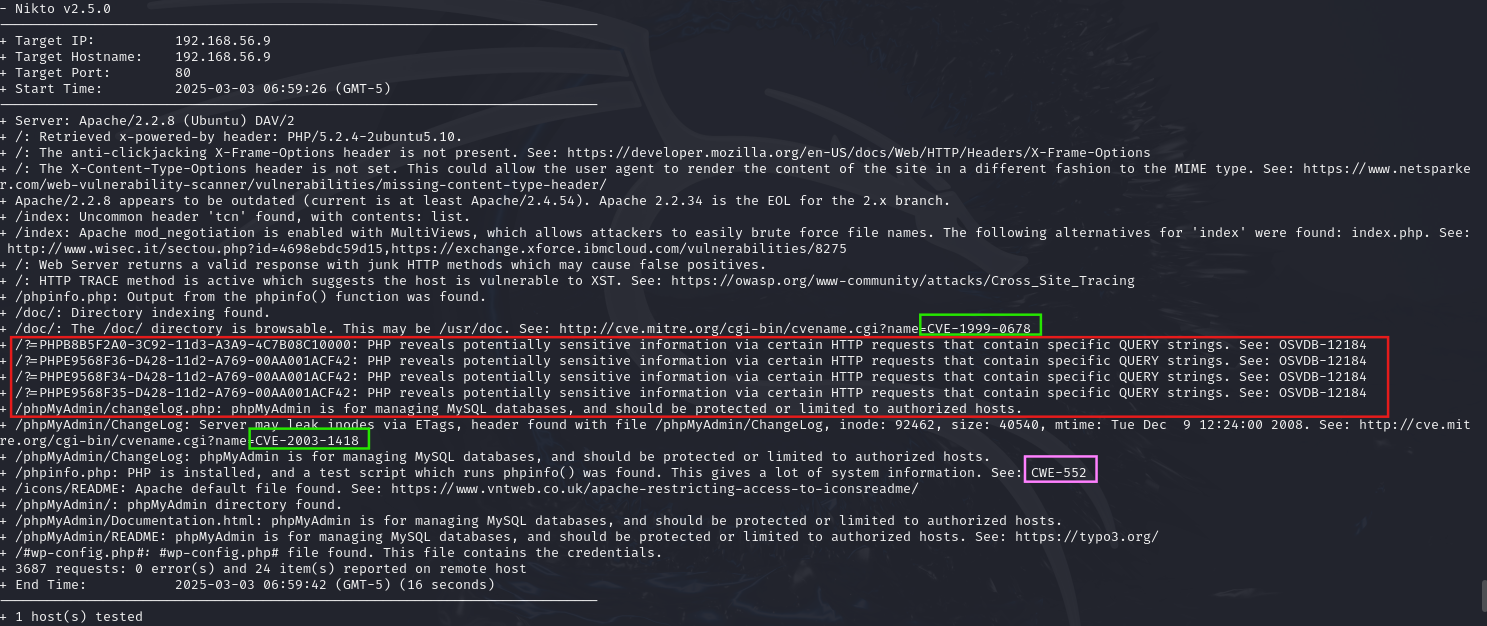
\includegraphics[width=1\textwidth]{imagenes/nikto.png}
             \caption{Herramienta \texttt{NIKTO} - puerto 80}
             \label{fig:nikto80}
            \end{figure}

        \item \textbf{Puerto 8180}. Este puerto está asociado con \texttt{Apache Tomcat} (Apache Tomcat/Coyote JSP engine 1.1). 
            \begin{figure} [hp!]
             \centering
             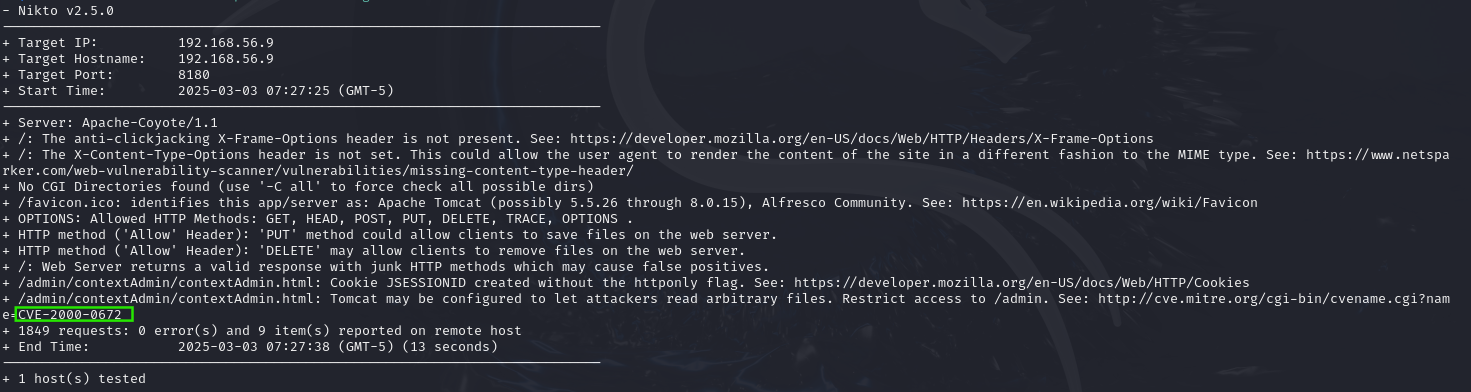
\includegraphics[width=1\textwidth]{imagenes/nikto8180.png}
             \caption{Herramienta \texttt{NIKTO} - puerto 8180}
             \label{fig:nikto8180}
            \end{figure}
    \end{itemize}


\newpage
\section{Identificación de Exploits}
\label{Apartado2}
En primer lugar, se usa la herramienta \texttt{SearchSploit} para encontrar los exploits relacionados con cada \texttt{CVE}, se realiza tanto para la máquina de Windows como la de Linux. A continuación,  basándonos en los resultados anteriores, se debe identificar al menos dos exploits para cada \texttt{CVE}, uno de ellos manual.

 \subsection{Identificación de Exploits - Máquina Windows (192.168.56.6)}

            \begin{figure} [hp!]
             \centering
             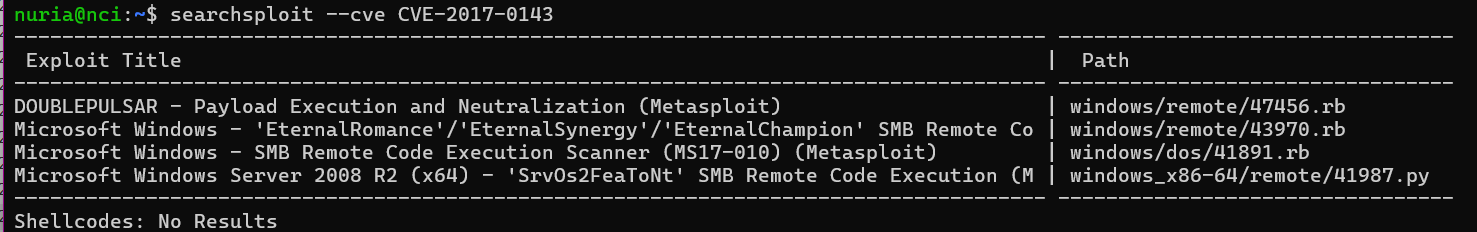
\includegraphics[width=1\textwidth]{imagenes/cve201743.png}
             \caption{ searchsploit --cve CVE-2017-0143}
             \label{fig:43}
            \end{figure}

            \begin{figure} [hp!]
             \centering
             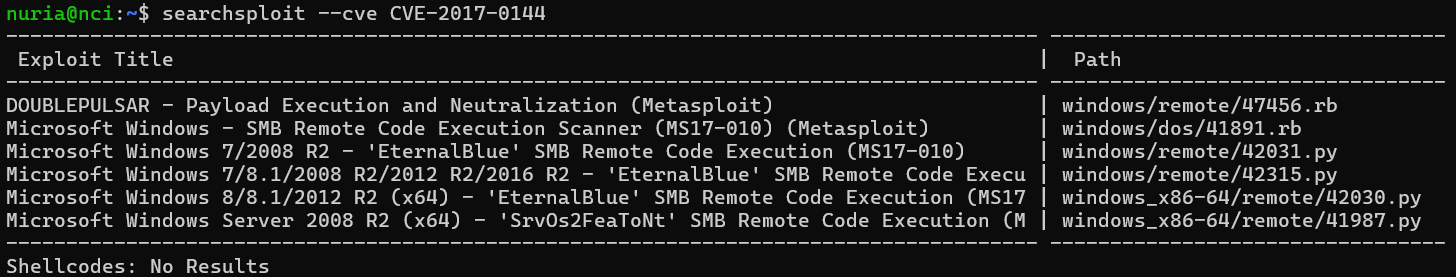
\includegraphics[width=1\textwidth]{imagenes/cve201744.png}
             \caption{ searchsploit --cve CVE-2017-0144}
             \label{fig:44}
            \end{figure}
            
            \begin{figure} [hp!]
             \centering
             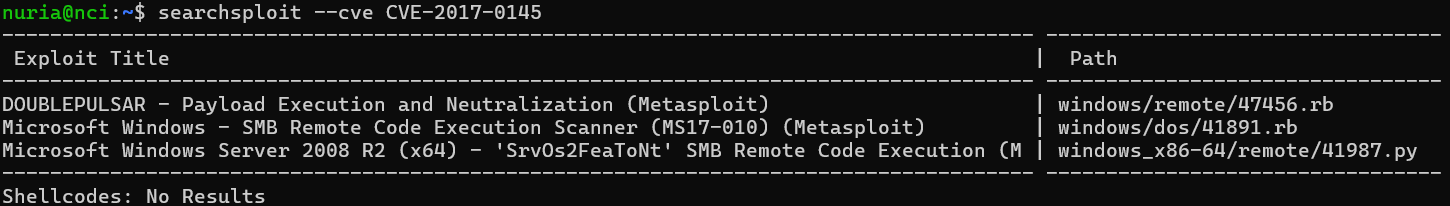
\includegraphics[width=1\textwidth]{imagenes/cve201745.png}
             \caption{ searchsploit --cve CVE-2017-0145}
             \label{fig:45}
            \end{figure}

            \begin{figure} [hp!]
             \centering
             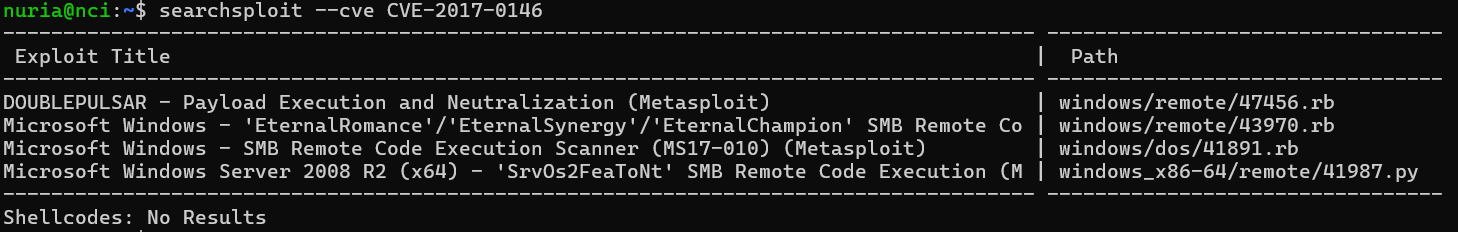
\includegraphics[width=1\textwidth]{imagenes/cve201746.png}
             \caption{ searchsploit --cve CVE-2017-0146}
             \label{fig:46}
            \end{figure}

\newpage
            \begin{figure} [hp!]
             \centering
             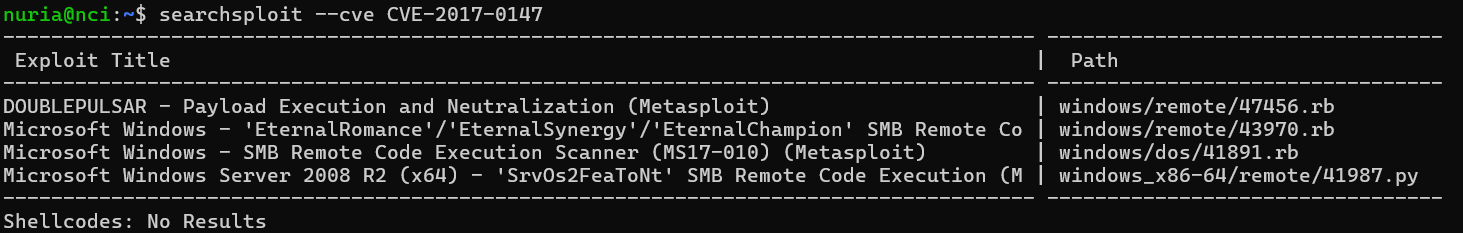
\includegraphics[width=1\textwidth]{imagenes/cve201747.png}
             \caption{ searchsploit --cve CVE-2017-0147}
             \label{fig:47}
            \end{figure}

            \begin{figure} [hp!]
             \centering
             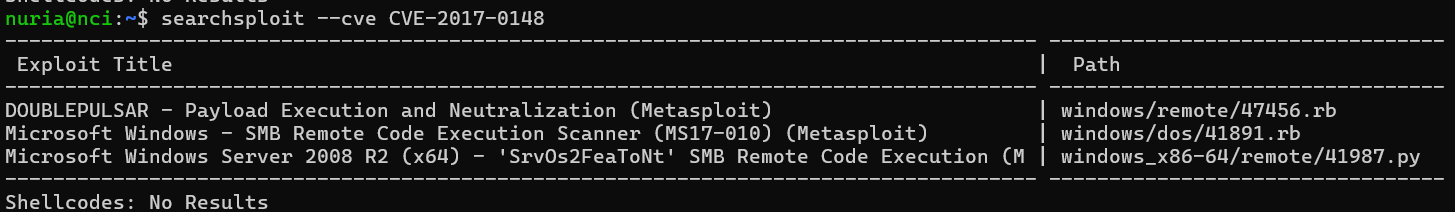
\includegraphics[width=1\textwidth]{imagenes/cve201748.png}
             \caption{ searchsploit --cve CVE-2017-0148}
             \label{fig:48}
            \end{figure}

            \begin{figure} [hp!]
             \centering
             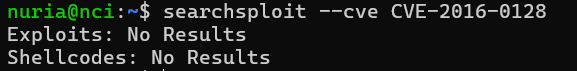
\includegraphics[width=0.6\textwidth]{imagenes/cve2016No.png}
             \caption{ searchsploit --cve CVE-2016-0128}
             \label{fig:16No}
            \end{figure}

            \begin{figure} [hp!]
             \centering
             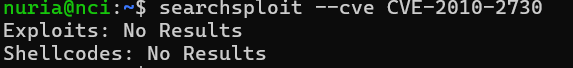
\includegraphics[width=0.6\textwidth]{imagenes/cve10No.png}
             \caption{ searchsploit --cve CVE-2010-2730}
             \label{fig:10No}
            \end{figure}
            
            \begin{figure} [hp!]
             \centering
             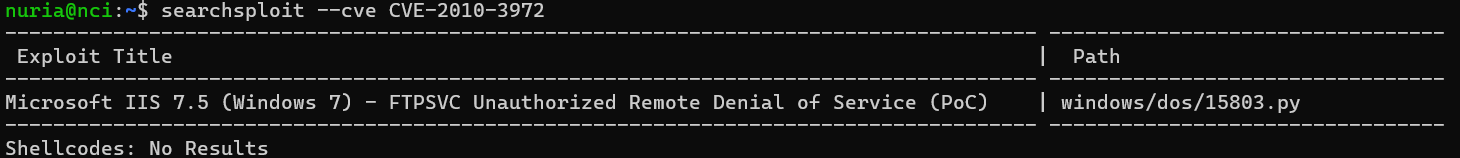
\includegraphics[width=1\textwidth]{imagenes/cve1072.png}
             \caption{ searchsploit --cve CVE-2010-3972}
             \label{fig:1072}
            \end{figure}
            
            \begin{figure} [hp!]
             \centering
             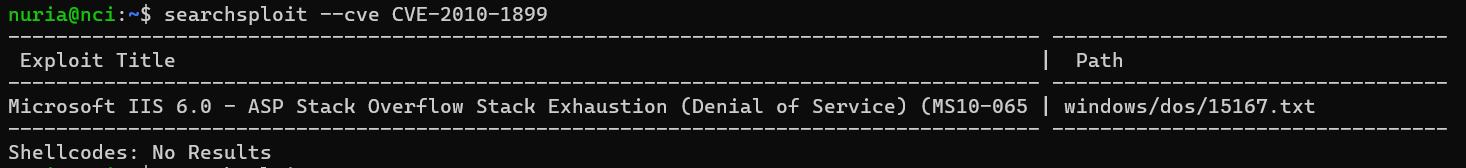
\includegraphics[width=1\textwidth]{imagenes/cve1089.png}
             \caption{ searchsploit --cve  CVE-2010-1899}
             \label{fig:1089}
            \end{figure}

\newpage
            \begin{figure} [hp!]
             \centering
             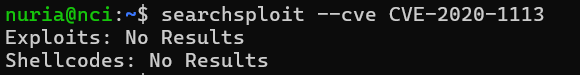
\includegraphics[width=0.6\textwidth]{imagenes/cve20No.png}
             \caption{ searchsploit --cve CVE-2020-1113}
             \label{fig:20No}
            \end{figure}

            \begin{figure} [hp!]
             \centering
             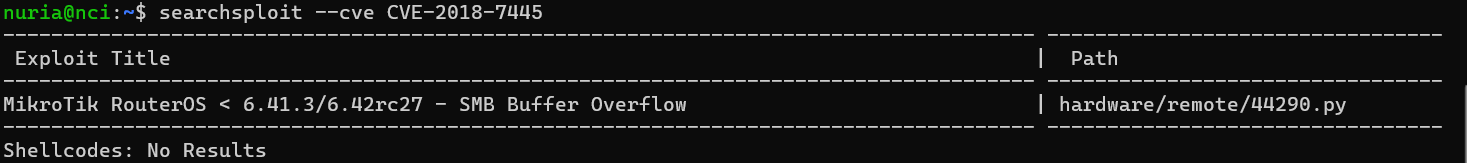
\includegraphics[width=1\textwidth]{imagenes/cve1845.png}
             \caption{ searchsploit --cve CVE-2018-7445}
             \label{fig:1845}
            \end{figure}

\subsubsection{Peligrosidad - exploits.}

\paragraph{Para cada exploit propuesto se debe indicar, en caso de que así sea, si el exploit supone algún peligro durante su ejecución (tipo BSOD) y en qué consiste.}


A partir de los exploits identificados en las vulnerabilidades listadas en las tablas \ref{tab:windows1} y \ref{tab:windows2} (principalmente relacionadas con el protocolo SMBv1 y otros fallos de software),en general, ninguno de los exploits detallados provoca directamente un BSOD en el sistema afectado, excepto en el caso de los relacionados con la vulnerabilidad CVE-2017-0143 (ETERNALBLUE). En este último caso, el exploit ( \texttt{Microsoft Windows Server 2008 R2 (x64) - ’SrvOs2FeaToNt’ SMB Remote Code Execution (MS17-010)}) puede provocar un BSOD debido a la ejecución de código malicioso en el núcleo del sistema, afectando la forma en que el protocolo SMB maneja las solicitudes de red.

\newpage

 \subsection{Identificación de Exploits - Máquina Linux (192.168.56.9)}

            \begin{figure} [hp!]
             \centering
             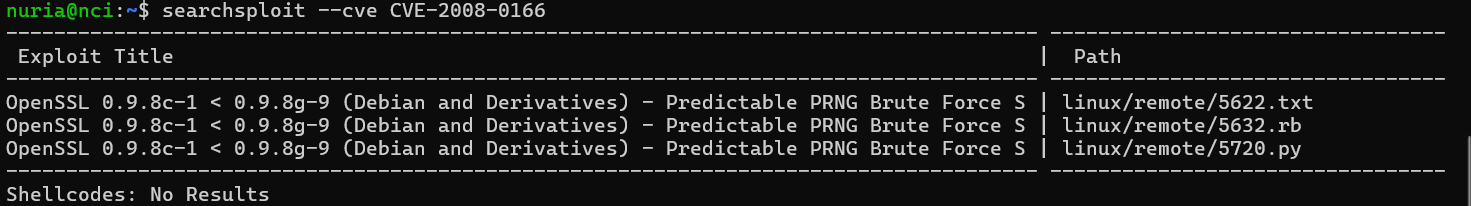
\includegraphics[width=1\textwidth]{imagenes/cvelinux1.png}
             \caption{ searchsploit --cve  CVE-2008-0166}
             \label{fig:linux1}
            \end{figure}

            \begin{figure} [hp!]
             \centering
             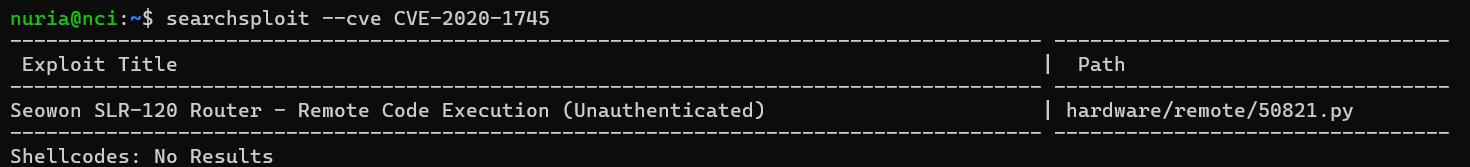
\includegraphics[width=1\textwidth]{imagenes/cvelinux2.png}
             \caption{ searchsploit --cve CVE-2020-1745}
             \label{fig:linux2}
            \end{figure}

            \begin{figure} [hp!]
             \centering
             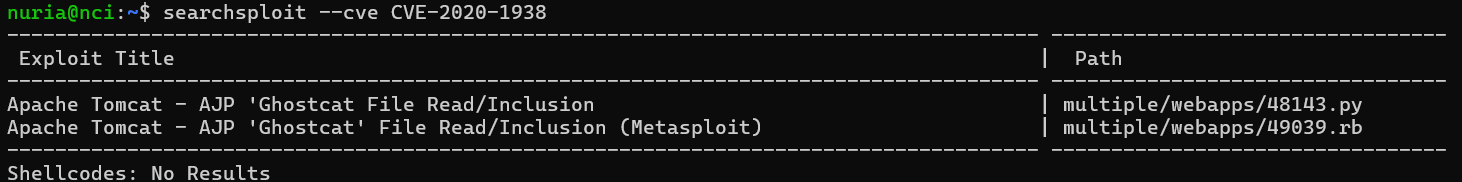
\includegraphics[width=1\textwidth]{imagenes/cvelinux3.png}
             \caption{ searchsploit --cve CVE-2020-1938}
             \label{fig:linux3}
            \end{figure}

            \begin{figure} [hp!]
             \centering
             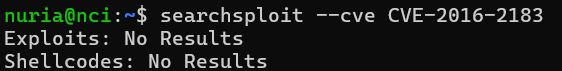
\includegraphics[width=0.6\textwidth]{imagenes/cvelinux4.png}
             \caption{ searchsploit --cve CVE-2016-2183}
             \label{fig:linux4}
            \end{figure}
        
            \begin{figure} [hp!]
             \centering
             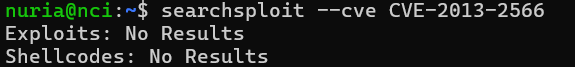
\includegraphics[width=0.6\textwidth]{imagenes/cvelinux5.png}
             \caption{ searchsploit --cve CVE-2013-2566}
             \label{fig:linux5}
            \end{figure}

            \begin{figure} [hp!]
             \centering
             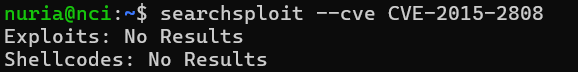
\includegraphics[width=0.6\textwidth]{imagenes/cvelinux6.png}
             \caption{ searchsploit --cve CVE-2015-2808}
             \label{fig:linux6}
            \end{figure}

            \begin{figure} [hp!]
             \centering
             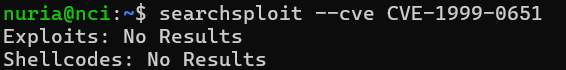
\includegraphics[width=0.6\textwidth]{imagenes/cvelinux7.png}
             \caption{ searchsploit --cve CVE-1999-0651}
             \label{fig:linux7}
            \end{figure}

\newpage

            \begin{figure} [hp!]
             \centering
             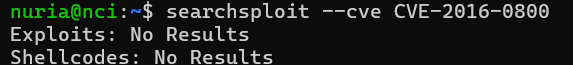
\includegraphics[width=0.6\textwidth]{imagenes/cvelinux8.png}
             \caption{ searchsploit --cve CVE-2016-0800}
             \label{fig:linux8}
            \end{figure}

            \begin{figure} [hp!]
             \centering
             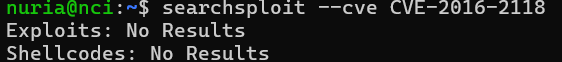
\includegraphics[width=0.6\textwidth]{imagenes/cvelinux9.png}
             \caption{ searchsploit --cve CVE-2016-2118}
             \label{fig:linux9}
            \end{figure}

            \begin{figure} [hp!]
             \centering
             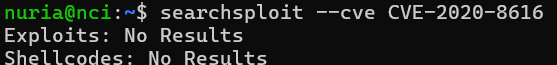
\includegraphics[width=0.6\textwidth]{imagenes/cvelinux10.png}
             \caption{ searchsploit --cve CVE-2020-8616}
             \label{fig:linux10}
            \end{figure}

            \begin{figure} [hp!]
             \centering
             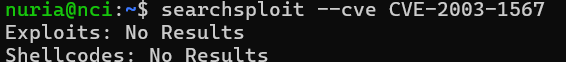
\includegraphics[width=0.6\textwidth]{imagenes/cvelinux11.png}
             \caption{ searchsploit --cve CVE-2003-1567}
             \label{fig:linux11}
            \end{figure}

            \begin{figure} [hp!]
             \centering
             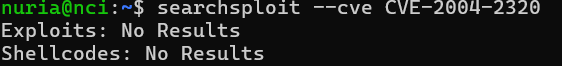
\includegraphics[width=0.6\textwidth]{imagenes/cvelinux12.png}
             \caption{ searchsploit --cve  CVE-2004-2320}
             \label{fig:linux12}
            \end{figure}


            \begin{figure} [hp!]
             \centering
             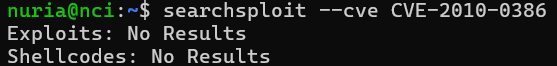
\includegraphics[width=0.6\textwidth]{imagenes/cvelinux13.png}
             \caption{ searchsploit --cve CVE-2010-0386}
             \label{fig:linux13}
            \end{figure}

\newpage
            \begin{figure} [hp!]
             \centering
             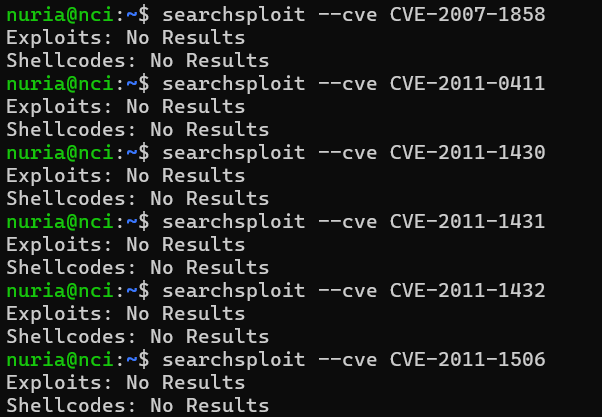
\includegraphics[width=0.6\textwidth]{imagenes/cvelinux14.png}
             \caption{ searchsploit --cve ...}
             \label{fig:linux14}
            \end{figure}

            \begin{figure} [hp!]
             \centering
             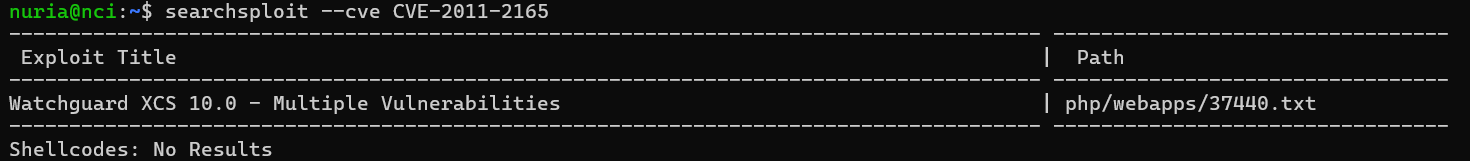
\includegraphics[width=1\textwidth]{imagenes/cvelinux15.png}
             \caption{ searchsploit --cve CVE-2011-2165}
             \label{fig:linux15}
            \end{figure}

            \begin{figure} [hp!]
             \centering
             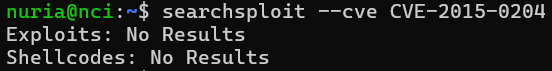
\includegraphics[width=0.6\textwidth]{imagenes/cvelinux16.png}
             \caption{ searchsploit --cve CVE-2015-0204}
             \label{fig:linux16}
            \end{figure}

            \begin{figure} [hp!]
             \centering
             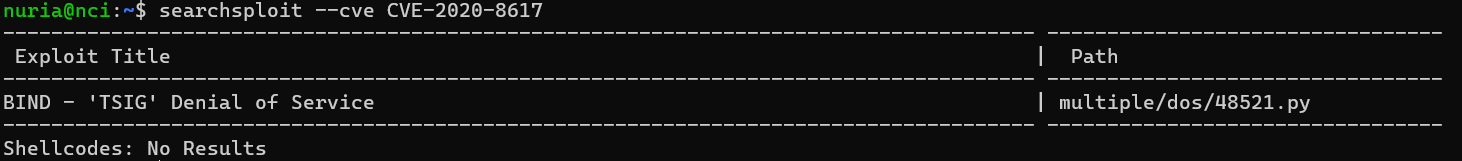
\includegraphics[width=1\textwidth]{imagenes/cvelinux17.png}
             \caption{ searchsploit --cve CVE-2020-8617}
             \label{fig:linux17}
            \end{figure}

\newpage
            \begin{figure} [hp!]
             \centering
             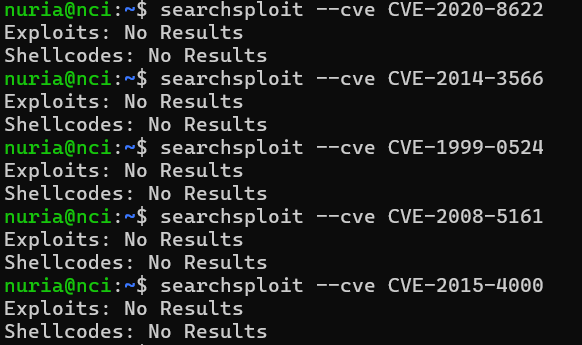
\includegraphics[width=0.6\textwidth]{imagenes/cvelinux18.png}
             \caption{ searchsploit --cve ...}
             \label{fig:linux18}
            \end{figure}

            \begin{figure} [hp!]
             \centering
             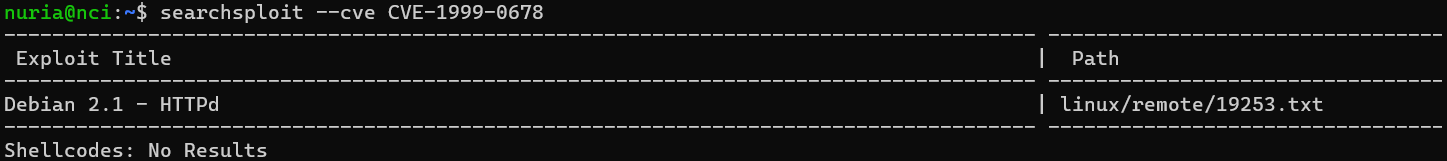
\includegraphics[width=1\textwidth]{imagenes/cvelinux19.png}
             \caption{ searchsploit --cve CVE-1999-0678}
             \label{fig:linux19}
            \end{figure}

            \begin{figure} [hp!]
             \centering
             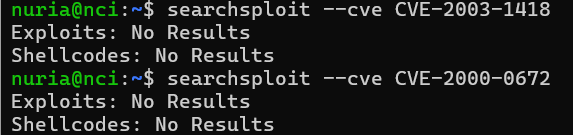
\includegraphics[width=0.6\textwidth]{imagenes/cvelinux20.png}
             \caption{ searchsploit --cve ...}
             \label{fig:linux20}
            \end{figure}

            \begin{figure} [hp!]
             \centering
             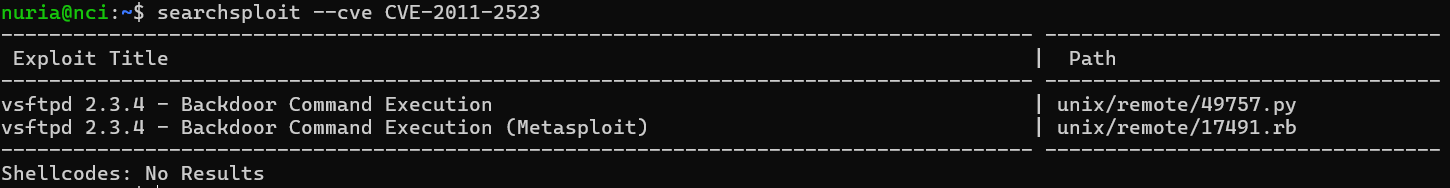
\includegraphics[width=1\textwidth]{imagenes/cvelinux21.png}
             \caption{ searchsploit --cve CVE-2011-2523}
             \label{fig:linux21}
            \end{figure}

            \begin{figure} [hp!]
             \centering
             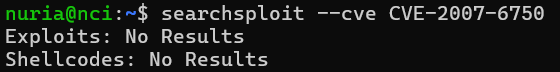
\includegraphics[width=0.6\textwidth]{imagenes/cvelinux22.png}
             \caption{ searchsploit --cve CVE-2007-6750}
             \label{fig:linux22}
            \end{figure}

\newpage
            \begin{figure} [hp!]
             \centering
             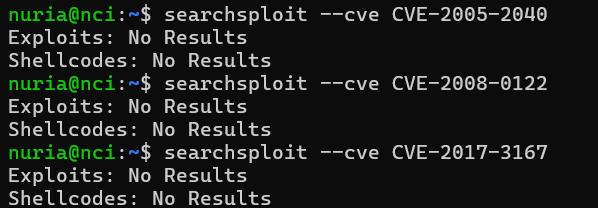
\includegraphics[width=0.6\textwidth]{imagenes/cvelinux23.png}
             \caption{ searchsploit --cve ...}
             \label{fig:linux23}
            \end{figure}

            \begin{figure} [hp!]
             \centering
             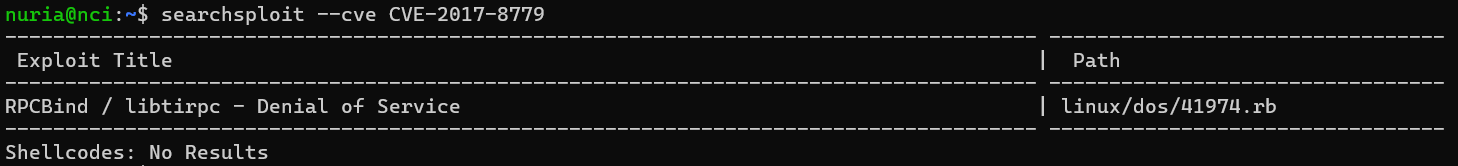
\includegraphics[width=1\textwidth]{imagenes/cvelinux24.png}
             \caption{ searchsploit --cve CVE-2017-8779}
             \label{fig:linux24}
            \end{figure}

            \begin{figure} [hp!]
             \centering
             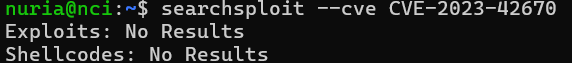
\includegraphics[width=0.6\textwidth]{imagenes/cvelinux25.png}
             \caption{ searchsploit --cve CVE-2023-42670}
             \label{fig:linux25}
            \end{figure}

            \begin{figure} [hp!]
             \centering
             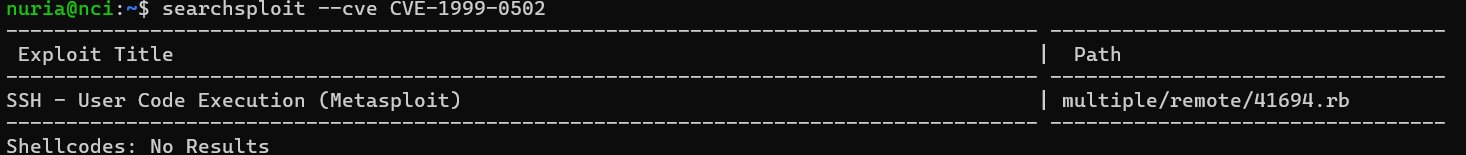
\includegraphics[width=1\textwidth]{imagenes/cvelinux26.png}
             \caption{ searchsploit --cve CVE-1999-0502}
             \label{fig:linux26}
            \end{figure}

            \begin{figure} [hp!]
             \centering
             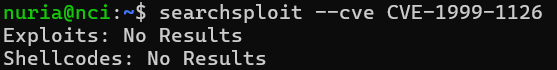
\includegraphics[width=0.6\textwidth]{imagenes/cvelinux27.png}
             \caption{ searchsploit --cve CVE-1999-1126}
             \label{fig:linux27}
            \end{figure}

            \begin{figure} [hp!]
             \centering
             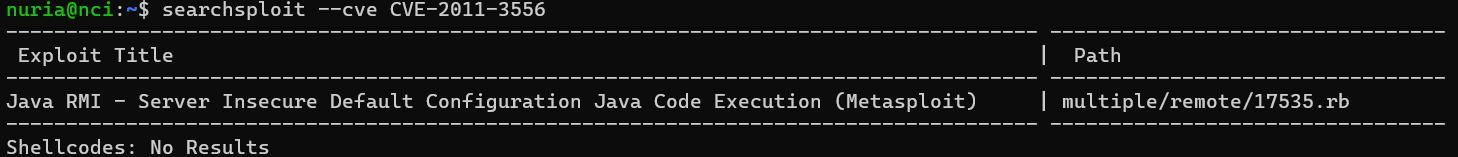
\includegraphics[width=1\textwidth]{imagenes/cvelinux28.png}
             \caption{ searchsploit --cve CVE-2011-3556}
             \label{fig:linux28}
            \end{figure}

\newpage
            \begin{figure} [hp!]
             \centering
             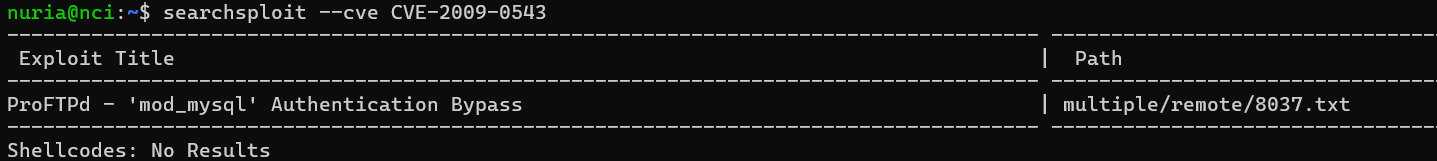
\includegraphics[width=1\textwidth]{imagenes/cvelinux29.png}
             \caption{ searchsploit --cve CVE-2009-0543}
             \label{fig:linux29}
            \end{figure}

            \begin{figure} [hp!]
             \centering
             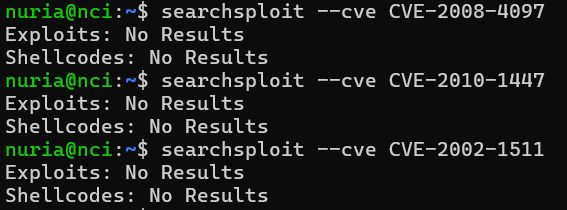
\includegraphics[width=0.6\textwidth]{imagenes/cvelinux30.png}
             \caption{ searchsploit --cve ...}
             \label{fig:linux30}
            \end{figure}


            \begin{figure} [hp!]
             \centering
             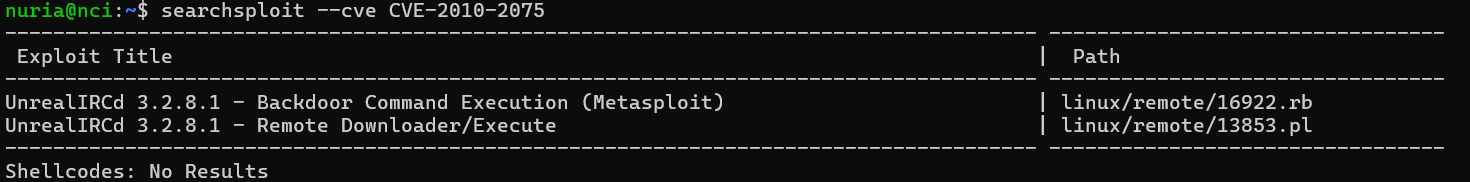
\includegraphics[width=1\textwidth]{imagenes/cvelinux31.png}
             \caption{ searchsploit --cve CVE-2010-2075}
             \label{fig:linux31}
            \end{figure}

            \begin{figure} [hp!]
             \centering
             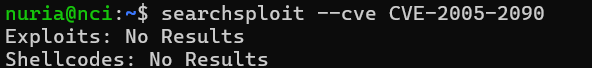
\includegraphics[width=0.6\textwidth]{imagenes/cvelinux32.png}
             \caption{ searchsploit --cve CVE-2005-2090}
             \label{fig:linux32}
            \end{figure}

\subsubsection{Peligrosidad - exploits.}

\paragraph{Para cada exploit propuesto se debe indicar, en caso de que así sea, si el exploit supone algún peligro durante su ejecución (tipo BSOD) y en qué consiste.}


A partir de los exploits identificados en las vulnerabilidades listadas en las tablas \ref{tab:linux1}, \ref{tab:linux2} y \ref{tab:linux3} (principalmente relacionadas con ejecución remota de código, ataques de denegación de servicio (DoS), y exposiciones de datos), ninguno de los exploits detallados en relación al S.O. Linux, provoca directamente un BSOD en el sistema afectado. En cambio, estos exploits comprometen principalmente la seguridad a nivel de software, lo que significa que pueden permitir la ejecución remota de código, la exposición de datos sensibles o ataques de denegación de servicio (DoS), pero no afectan directamente la estabilidad del sistema operativo.








\newpage
\section{Referencias}
\printbibliography[heading=none]

\end{document}
